%% tags: thickArrow
\PassOptionsToPackage{usenames,dvipsnames}{xcolor}
\documentclass[tikz,border=2]{standalone}
\usepackage{../cba}
\usepackage{amssymb}
\usepackage{enumerate}
\usepackage{mathtools} % contains amsmath which comes with align
\usepackage{amsthm}
\usepackage{graphicx}
\usepackage{microtype} % some compression
\usepackage[skins]{tcolorbox}
%%%%%%%%%%
% brown blue red
\definecolor{LightBlue}{HTML}{C7DFE3}
\definecolor{DarkBlue}{HTML}{72AFB6}
\definecolor{DarkBrown}{HTML}{D2BE89}
\definecolor{LightBrown}{HTML}{F4ECDF}
\definecolor{Grey}{HTML}{A7A195}
%%\definecolor{Red}{HTML}{CA6C2E}
%%
\usetikzlibrary{shadows,arrows.meta,arrows,shapes,positioning,calc,backgrounds,
fit,automata,decorations.markings,
decorations.pathreplacing,decorations.pathmorphing}
%%%%%%%%%%%%%%%%%%%%%%%
\begin{document}
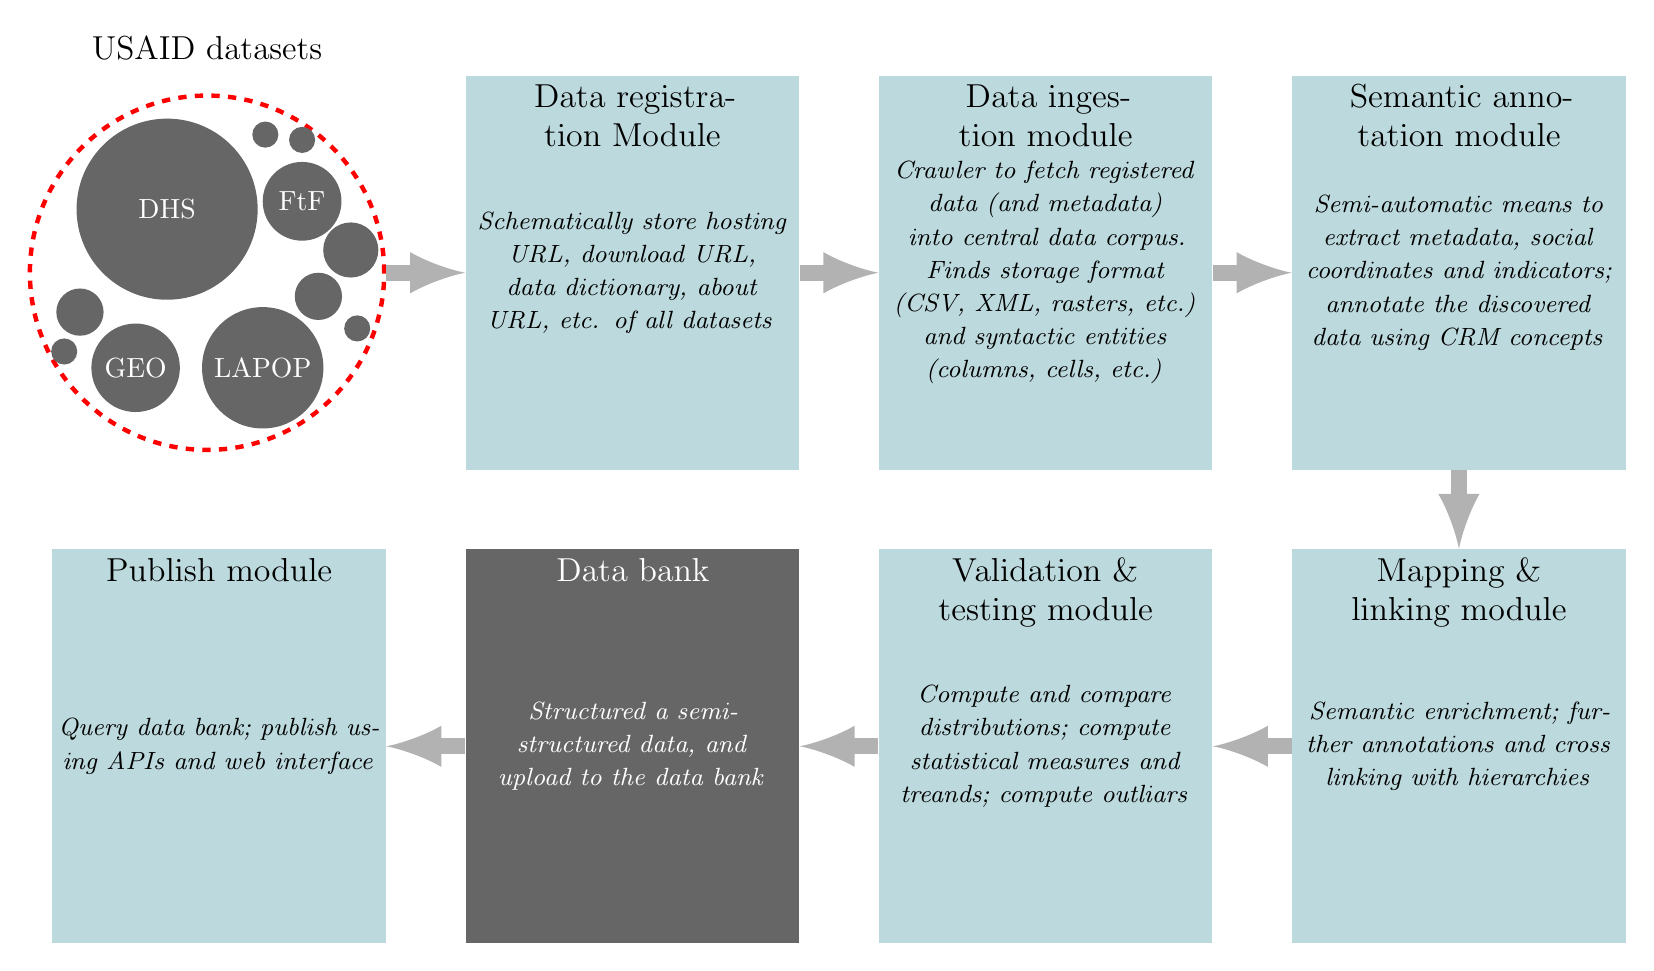
\begin{tikzpicture}
[scale=1,auto, transform shape,
   node distance=1cm,
every node/.style={align=center},
source/.style={circle,text=white,fill=Gray!120},
module/.style={rectangle,minimum height=5cm,minimum
width=4cm,text=black,fill=LightBlue!120, text width=4cm},
titleBlock/.style={anchor=north,font=\large,text width=3.5cm},
submodule/.style={node distance=.7cm,rectangle,minimum width=1.3cm, text width=1.3cm, anchor=south,draw},
meta/.style={dashed,font,rectangle,rounded corners,minimum width=2cm,text=Gray},
myedge/.style={draw=Gray!60,>=latex, shorten >=.0pt, shorten <=.0pt, 
line width=2mm}]
%%%%%%%%%%%%%%%%
% Modules
%%%%%%%%%%%%%%%%
%% usaid
\node (usaid) [circle,minimum width=4.5cm,dashed,font=\large,draw=red,ultra
thick] at (0,0) {};
\node [above=of usaid,font=\large,shift={(0,-.7cm)}] {USAID datasets};
\node (dhs) [source,above left of=usaid,shift={(.2,.1)},minimum width=2.3cm] {DHS};
\node (ftf) [source,above right of=usaid,shift={(.5,+0.2)},minimum width=1cm] {FtF};
\node (lapop) [source,below right of=usaid,shift={(0,-0.5)},minimum width=1.5cm] {LAPOP};
\node (geo) [source,below left of=usaid,shift={(-.2,-0.5)}] {GEO};
\node (m1) [source,above right= of dhs,shift={(-.4,-0.7)}] {};
\node (m2) [source,above=of ftf,shift={(0,-0.9)}] {};
\node (m2) [source,below right=of ftf,minimum width=.7cm,shift={(-.7,.7)}] {};
\node (m3) [source,above left of=geo,minimum width=.6cm,shift={(0,0)}] {};
\node (m4) [source,above left of=geo,shift={(-.2,-0.5)}] {};
\node (m5) [source,right of=lapop,shift={(.2,0.5)}] {};
\node (m5) [source,above right of=lapop,minimum width=.6cm,shift={(0,.2)}] {};
%% data retrieval
\node (retrieve) [module,right=of usaid] {\textit {\small Schematically store hosting URL, download URL, data dictionary, about URL, etc. of all datasets}};
\node at (retrieve.north) [titleBlock] {Data registration Module};
%% data ingestion
\node (ingest) [module,right=of retrieve] {\textit {\small Crawler to fetch registered data (and metadata) into central data corpus. Finds storage format (CSV, XML, rasters, etc.) and syntactic entities (columns, cells, etc.)}};
\node at (ingest.north) [titleBlock] {Data ingestion module};
%% data ingestion
\node (annotate) [module,right=of ingest] {\textit {\small Semi-automatic means to extract metadata, social coordinates and indicators; annotate the discovered data using CRM concepts }};
\node at (annotate.north) [titleBlock] {Semantic annotation module};
%% mapping & linking
\node (maplink) [module,below=of annotate] {\textit {\small Semantic enrichment; further annotations and cross linking with hierarchies}};
\node at (maplink.north) [titleBlock] {Mapping \& linking module};
%% Validation & testing
\node (validate) [module,left=of maplink] {\textit {\small Compute and compare distributions; compute statistical measures and treands; compute outliars}};
\node at (validate.north) [titleBlock] {Validation \& testing module};
%% Data bank
\node (bank) [module,fill=Gray!120,text=white,left=of validate] {\textit {\small
Structured a semi-structured data, and upload to the data bank}};
\node at (bank.north) [titleBlock,text=white,] {Data bank};
%% Publish module
\node (publish) [module,left=of bank] {\textit {\small Query data bank; publish using APIs and web interface}};
\node at (publish.north) [titleBlock] {Publish module};


%%%%%%%%%%%%%%%%
% arrows
%%%%%%%%%%%%%%%%
\draw[myedge,->] (usaid) -- (retrieve);
\draw[myedge,->] (retrieve) -- (ingest);
\draw[myedge,->] (ingest) -- (annotate);
\draw[myedge,->] (annotate) -- (maplink);
\draw[myedge,->] (maplink) -- (validate);
\draw[myedge,->] (validate) -- (bank);
\draw[myedge,->] (bank) -- (publish);
\end{tikzpicture}
\end{document}
